\hfil
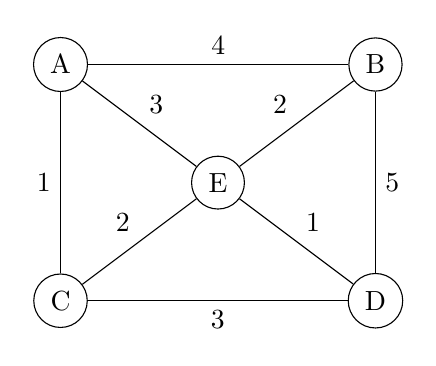
\begin{tikzpicture}
    \begin{scope}[grow'=right,
        every node/.style = {shape=circle, draw, align=center},
        every tree node/.style={anchor=base west}]
        \node (A) at (0,1.5) {A};
        \node (B) at (4,1.5) {B};
        \node (C) at (0,-1.5) {C};
        \node (D) at (4,-1.5) {D};
        \node (E) at (2,0) {E};
    \end{scope}

    \begin{scope}
    \path [-] (A) edge node[above]{4} (B);
    \path [-] (A) edge node[left]{1} (C);
    \path [-] (A) edge node[above right] {3} (E);
    \path [-] (B) edge node[right] {5} (D);
    \path [-] (B) edge node[above left] {2} (E);
    \path [-] (C) edge node[above left] {2} (E);
    \path [-] (C) edge node[below] {3} (D);
    \path [-] (D) edge node[above right] {1} (E);
    \end{scope}

  \end{tikzpicture}